\newpage
\chapter{Face-Clustering-Based Method for Educational Video Recommendation}
\label{chap:educational_recommendation}

It is a common practice among educational content creators to make collaborative videos, that is, videos in which more than one lecturer is presenting the lecture content.
Such collaborations create a network of lecturers teaching a given subject.
Therefore, a method that identifies these collaborations may help students find their content of interest more easily.
In this chapter, we describe the second application we investigated using our \emph{Video Face Clustering} method.
We propose a recommender method based on the actor's presence for educational videos. In this case, the actors are lecturers~(or teachers, professors, etc.) that are presenting educational content on video.
For instance, if a student watches a video containing lecturers A and B, our method aims at recommending other videos that contain at least one of these lecturers. 
This method provides an additional aid for educational recommender systems, allowing them to use the presence of lecturers as a feature for composing their recommendations.

The remainder of this chapter is structured as follows.
Section~\ref{sec:recommendation_dataset} presents the dataset we used.
We present our method in Section~\ref{sec:recommendation_method}, followed by 
Section~\ref{sec:recommendation_ranking_evaluation}, that shows the experiments to evaluate our recommendation ranking mechanisms.
Finally, in Section~\ref{sec:recommendation_discussion}, we conclude this chapter by discussing our results.

\section{Dataset}
\label{sec:recommendation_dataset}

The experiments were conducted using a dataset created in the context of this application.
It is composed of 98 educational videos publicly available on YouTube.\footnote{\url{https://www.youtube.com/channel/UCT0JugAtGmqiYkwxFZOwAtg}}$^{,}$\footnote{\url{https://www.youtube.com/user/deboraaladim}}
Each video contains at least one lecturer; moreover, some videos could have some special participation or collaboration. Therefore, the number of lecturers in each video varies from 1 to 5. In total, 16 different lecturers are present in the dataset. Each lecturer is present, on average, in 6.67\% of the videos.
We also annotated the name of each lecturer present in the videos, so that we can verify if correct videos are being recommended.

%%
The videos duration vary from 00m:30s to 1h:49m:01s. 
The average duration of the videos is 23m:34s, with a standard deviation of 23m:05s. 
The high value of the standard deviation for the time estimates indicates that the videos are not in the same time range, and therefore have a wide duration variety. 

\section{Proposed Method}
\label{sec:recommendation_method}

Our method intends to recommend educational videos based on the lecturers that appear in each video, so that, when a person watches a video, other videos containing the same lecturers are recommended.
For doing that, we first represent each video in the dataset of educational videos by the clusters of lecturers present using \emph{Video Face Clustering}. Once we have all videos represented, we perform the pipeline depicted in Figure \ref{fig:video_recommendation}. Each of the steps of this pipeline is described in the remainder of this section.

\begin{figure}[!ht]
  \centering
  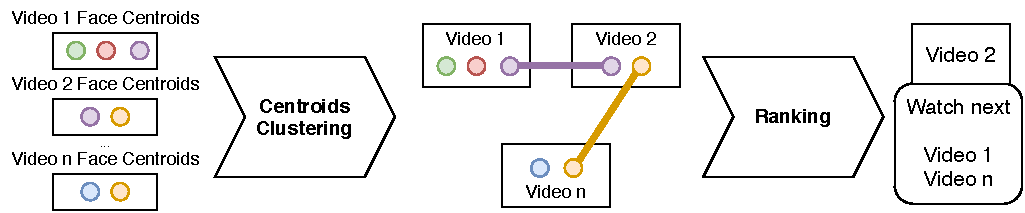
\includegraphics[width=1\textwidth]{img/video_recommendation/video_recommendation.pdf}
  \caption{Video Recommendation based on Lecturers Centroids Clustering}
  \label{fig:video_recommendation}
\end{figure}

First, we gather the centroids from the videos of the dataset as one single set and perform the \textit{Centroids Clustering}.
For performing this clustering, we also use the strategy for an unknown number of clusters described in Section \ref{subsec:unknown_nclusters}. 
By doing that, we group centroids from the same lecturer that are in different videos. For instance, in Figure \ref{fig:video_recommendation}, one can see that the \emph{purple lecturer} is present in both Videos 1 and 2, while the \emph{orange lecturer} is present in both Videos 2 and n. By the end of this step, we have the group $L$ of lecturers present in the dataset of videos $V$. We also denote $L_v$ as the group of lecturers present in video $v$.

Next, based on these relationships among different videos, we perform \textit{Ranking}, by recommending videos in which lecturers of the current video are present. 
For doing that, we compute a similarity score using the presence of the lecturers in the current video and the presence of these same lecturers in the other video.
Let $p_{l,v}$ denote the percentage of frames in which the lecturer $l \in L_v$ is present in video $v \in V$. For each video $v \in V$ and $u \in V-v$ we compute a score of similarity $S_{v,u}$.

\begin{equation}
  S_{v,u} = \sum_{l~\in~L_v}{p_{l,v}\cdot{p_{l,u}}}
\end{equation}

Finally, using this score, for each video $v$ we compute a ranking $R_{v}$ where $R_{v,i}$ denotes the \emph{i-greatest} $S_v$ and $R_{v,i}\ge~R_{v,i+1}$ for all $i~\in~1...n_v$, where $n_v$ is the number of videos $u$ in which $S_{v,u}>~0$. 
In this way, the more lecturers a video has in common with the reference video, and the more time these lecturers are present in both videos, the higher the video is positioned in the ranking of the reference video.  

By the end of this phase, we have a ranking of recommended videos for each video in the dataset.
It is important to notice that our method is unsupervised and does not require the information of the lecturers in advance.
Consequently, we do not have to store any information regarding the identity of the lecturers, respecting their privacy.


\section{Ranking Evaluation}
\label{sec:recommendation_ranking_evaluation}

This section describes an experiment we conducted for evaluating how well our recommendation approach performed in terms of recommending relevant videos. We define that a recommendation is relevant if the reference and the recommended video have at least one lecturer in common.

First, we compute the clusters that represent each lecturer in each video using \emph{Video Face Clustering}. 
We start by performing \emph{Frames Extraction} for each video file using a frame rate of 1 frame per second~(fps). 
Next, in the \emph{Face Detection} step, we use MTCNN \cite{mtcnn}.
Once we have detected the faces of lecturers in the video frames, we perform \emph{Embeddings Generation} using SeNet-50 \cite{senet} that generates embeddings on the $\mathbb{R}^{2048}$ feature space. 
We used the architecture and weights pre-trained on the VGGFace2 dataset~\cite{cao2018vggface2}.
Finally, in the \emph{Clustering} step, since we do not know the number of clusters in advance, we used the strategy described in Section \ref{subsec:unknown_nclusters} with $t=5$, $\omega=0.2$, that empirically demonstrated good results. For the \texttt{Clustering} procedure, we used Agglomerative Clustering~\cite{ward1963hierarchical}.
The choice of using SeNet-50 and Agglomerative Clustering comes from the fact that this combination achieved the best results in the experiment described in Section \ref{sec:recognition_clustering_validation}.

For performing the video recommendation task, we gather the centroids~(that represent each lecturer in the video) from all videos in the dataset. Next, we perform the process described in Section \ref{sec:recommendation_method}. For \emph{Centroids Clustering}, we also use Algorithm \ref{clustering_alg} with the same parameters $t=5$, $\omega=0.2$, and the Aglommerative Clustering as \texttt{Clustering} procedure. Finally, based on the clusters generated, we perform the \emph{Ranking} step

To evaluate our ranking, for each video we compute the Average Precision~(AP), which evaluates how well a ranking of recommendations is based on each element's relevancy. 
This metric penalizes more a ranking if a non-relevant element is recommended in the first positions than if it was in the last ones.
Let $P_k$ be the precision of the first $k$ elements of a ranking, which is the percentage of videos that are relevant in the sub-ranking that starts at position $1$ and ends at position $k$.
Let $\alpha_k$ denote the relevancy of the video in position $k$, where $\alpha_k = 1$ if the video is relevant, and $0$ otherwise.
The AP of a given ranking is defined as follows
\begin{equation}
  \label{equation:average_precision}
  AP = \frac{1}{GTP}\sum_{k=1}^{n}{P_k~\cdot~\alpha_k}
\end{equation}
where GTP refers to the total number of ground truth positives in the ranking, which is the total number of videos that are considered relevant in a ranking. Figure \ref{fig:ap_example} shows an example of how the AP is computed for a given ranking. In this case, the $GTP=3$ because the total number of relevant videos in the ranking is 3~(videos A, B and D).

\begin{figure}[ht]
  \centering
  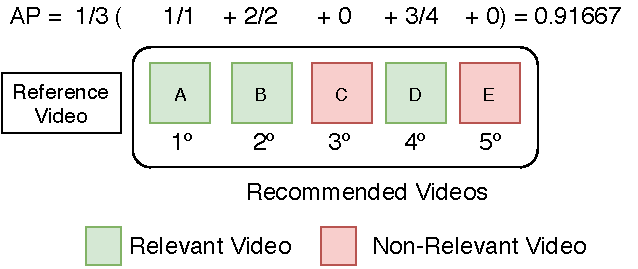
\includegraphics[width=0.7\linewidth]{img/video_recommendation/ap_example.pdf}
  \caption{Example of how the Average Precision~(AP) is computed for a reference video and its recommended videos.}
  \label{fig:ap_example}
\end{figure}

In order to prevent outliers from having much influence in the recommendation (e.g. a person that is not a lecturer -- and not relevant to the video -- and appears for a short amount of time), we experimented different thresholds of presence intervals in a video for a person to be considered as ``present'' when computing the score for the ranking. 
In this way, a $p_{l,v}$ lesser than the threshold is considered as $0$.
Besides the Average Precision, we also compute the mean and minimum values of the recall~(MeanR), precision~(MeanP), and F1-Score~(MeanF1) for the recommendation generated for each of the videos, without considering the positioning of these videos in the rankings.
The recall refers to the percentage of relevant videos that are present in the ranking.
The F1-score represents an overall performance metric based on the harmonic mean of the precision and recall.
Table \ref{tab:results} shows the thresholds used, the values of recall, precision, F1-score, and the Mean Average Precision (mAP).

One can observe from Table \ref{tab:results} that the precision increased with the use of the threshold.
Different from the precision, the recall decreased with the increase of the threshold. It means that with a greater threshold more videos that should be recommended were not chosen by our method.
It is important to notice that these two metrics~(precision and recall) do not consider the ordering of the recommendations.
Different from them, the Mean Average Precision~(mAP) has high values for all thresholds, especially because the score for computing the ranking takes into consideration the percentage of time that a person appears in the reference and recommended videos.
Then, we can conclude that our proposed approach for ordering the recommended videos tends to recommend more suitable videos first with a high mAP$\approx0.99$. 

\begin{table*}[!ht]
\small
\centering
\caption{Results obtained with our approach with different thresholds of time presence for a lecturer to be considered as present in a video.}
\label{tab:results}
\begin{tabular}{ccccc}
\hline
\textbf{Thershold} & \textbf{MeanR}  & \textbf{MeanP} & \textbf{MeanF1} &\textbf{mAP} \\ \hline
0\%                & 0,88851         & 0,64681        & 0,70971         & 0,98641   \\
1\%                & 0,88851         & 0,64681        & 0,70971         & 0,98641   \\
2\%                & 0,88851         & 0,64885        & 0,71171         & 0,98641   \\
3\%                & 0,88851         & 0,67368        & 0,73086         & 0,98642   \\
4\%                & 0,88851         & 0,67368        & 0,73086         & 0,98642   \\
5\%                & 0,88851         & 0,69923        & 0,74930         & 0,98642   \\
6\%                & 0,88851         & 0,73615        & 0,77648         & 0,98642   \\
7\%                & 0,88742         & 0,77849        & 0,80768         & 0,98642   \\
8\%                & 0,88742         & 0,78408        & 0,81111         & 0,98643   \\
9\%                & 0,88742         & 0,80171        & 0,82410         & 0,98643   \\
10\%               & 0,88742         & 0,83165        & 0,84306         & 0,98643   \\
11\%               & 0,88742         & 0,85306        & 0,85693         & 0,98643   \\
12\%               & 0,88616         & 0,85956        & 0,86018         & 0,98662   \\
13\%               & 0,88490         & 0,88216        & 0,87305         & 0,98688   \\
14\%               & 0,88289         & 0,90265        & 0,88450         & 0,98884   \\
15\%               & 0,88289         & 0,90265        & 0,88450         & 0,98884   \\
16\%               & 0,88163         & 0,91327        & 0,88980         & 0,98908   \\
17\%               & 0,87197         & 0,91538        & 0,88580         & 0,98912   \\
18\%               & 0,87197         & 0,91538        & 0,88580         & 0,98912   \\
19\%               & 0,87086         & 0,93165        & 0,89476         & 0,98946   \\
20\%               & 0,86130         & 0,93645        & 0,89218         & 0,99000   \\
21\%               & 0,86130         & 0,93645        & 0,89218         & 0,99000   \\
22\%               & 0,86130         & 0,95054        & 0,89886         & 0,99000   \\
23\%               & 0,86130         & 0,95054        & 0,89886         & 0,99000   \\
24\%               & 0,85805         & 0,95718        & 0,90046         & 0,99165   \\
25\%               & 0,85805         & 0,95718        & 0,90046         & 0,99165  
\end{tabular}
\end{table*}

\section{Discussion}
\label{sec:recommendation_discussion}

In this chapter, we present a method for educational video recommendation using \emph{Video Face Clustering}. More precisely, we use an unsupervised clustering-based method and a heuristic for ranking.
We extract the video face clusters centroids to perform another clustering step that creates a relationship of videos that share the presence of the same lecturers.
Finally, we rank the recommended videos based on the amount of time each lecturer is present.
It is worth mentioning that our method is completely automatic and does not require any information from the video files in advance.  
Moreover, our approach does not need to know or store the identity of the lecturers for performing recommendations, preserving their privacy.

A collateral contribution of this application, that is a result of \emph{Video Face Clustering}, is video segmentation by lecturers.
As illustrated in Figure \ref{fig:video_timeline}, we can create a timeline based on lecturers' presence, which can be used to help students in finding moments where specific lecturers are present.
With this segmentation, we could recommend specific parts of the video to the student.

\begin{figure}[!ht]
  \centering
  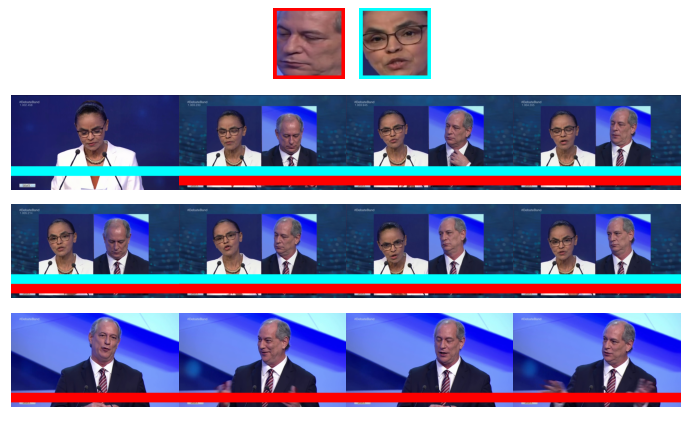
\includegraphics[width=0.8\linewidth]{img/face_clustering/example_localization.png}
  \caption{Educational video timeline tagged by the lecturers presence. Notice that the frames with the lecturer on the left are tagged in red, while the frames with the lecturer on the right are tagged in yellow.}
  \label{fig:video_timeline}
\end{figure}

The main limitation of our method is that we can only recommend videos in which the lecturers are visually present. However, this method can be used in a hybrid recommendation approach, that combines both textual and audiovisual information from the video to create clusters. 
The results of this application were published at relevant multimedia conference~\cite{mendes2020ISM}.